\documentclass[tikz,border=10pt]{standalone}
\usepackage{tikz}
\usetikzlibrary{automata,positioning,arrows.meta,shapes.geometric}

\begin{document}
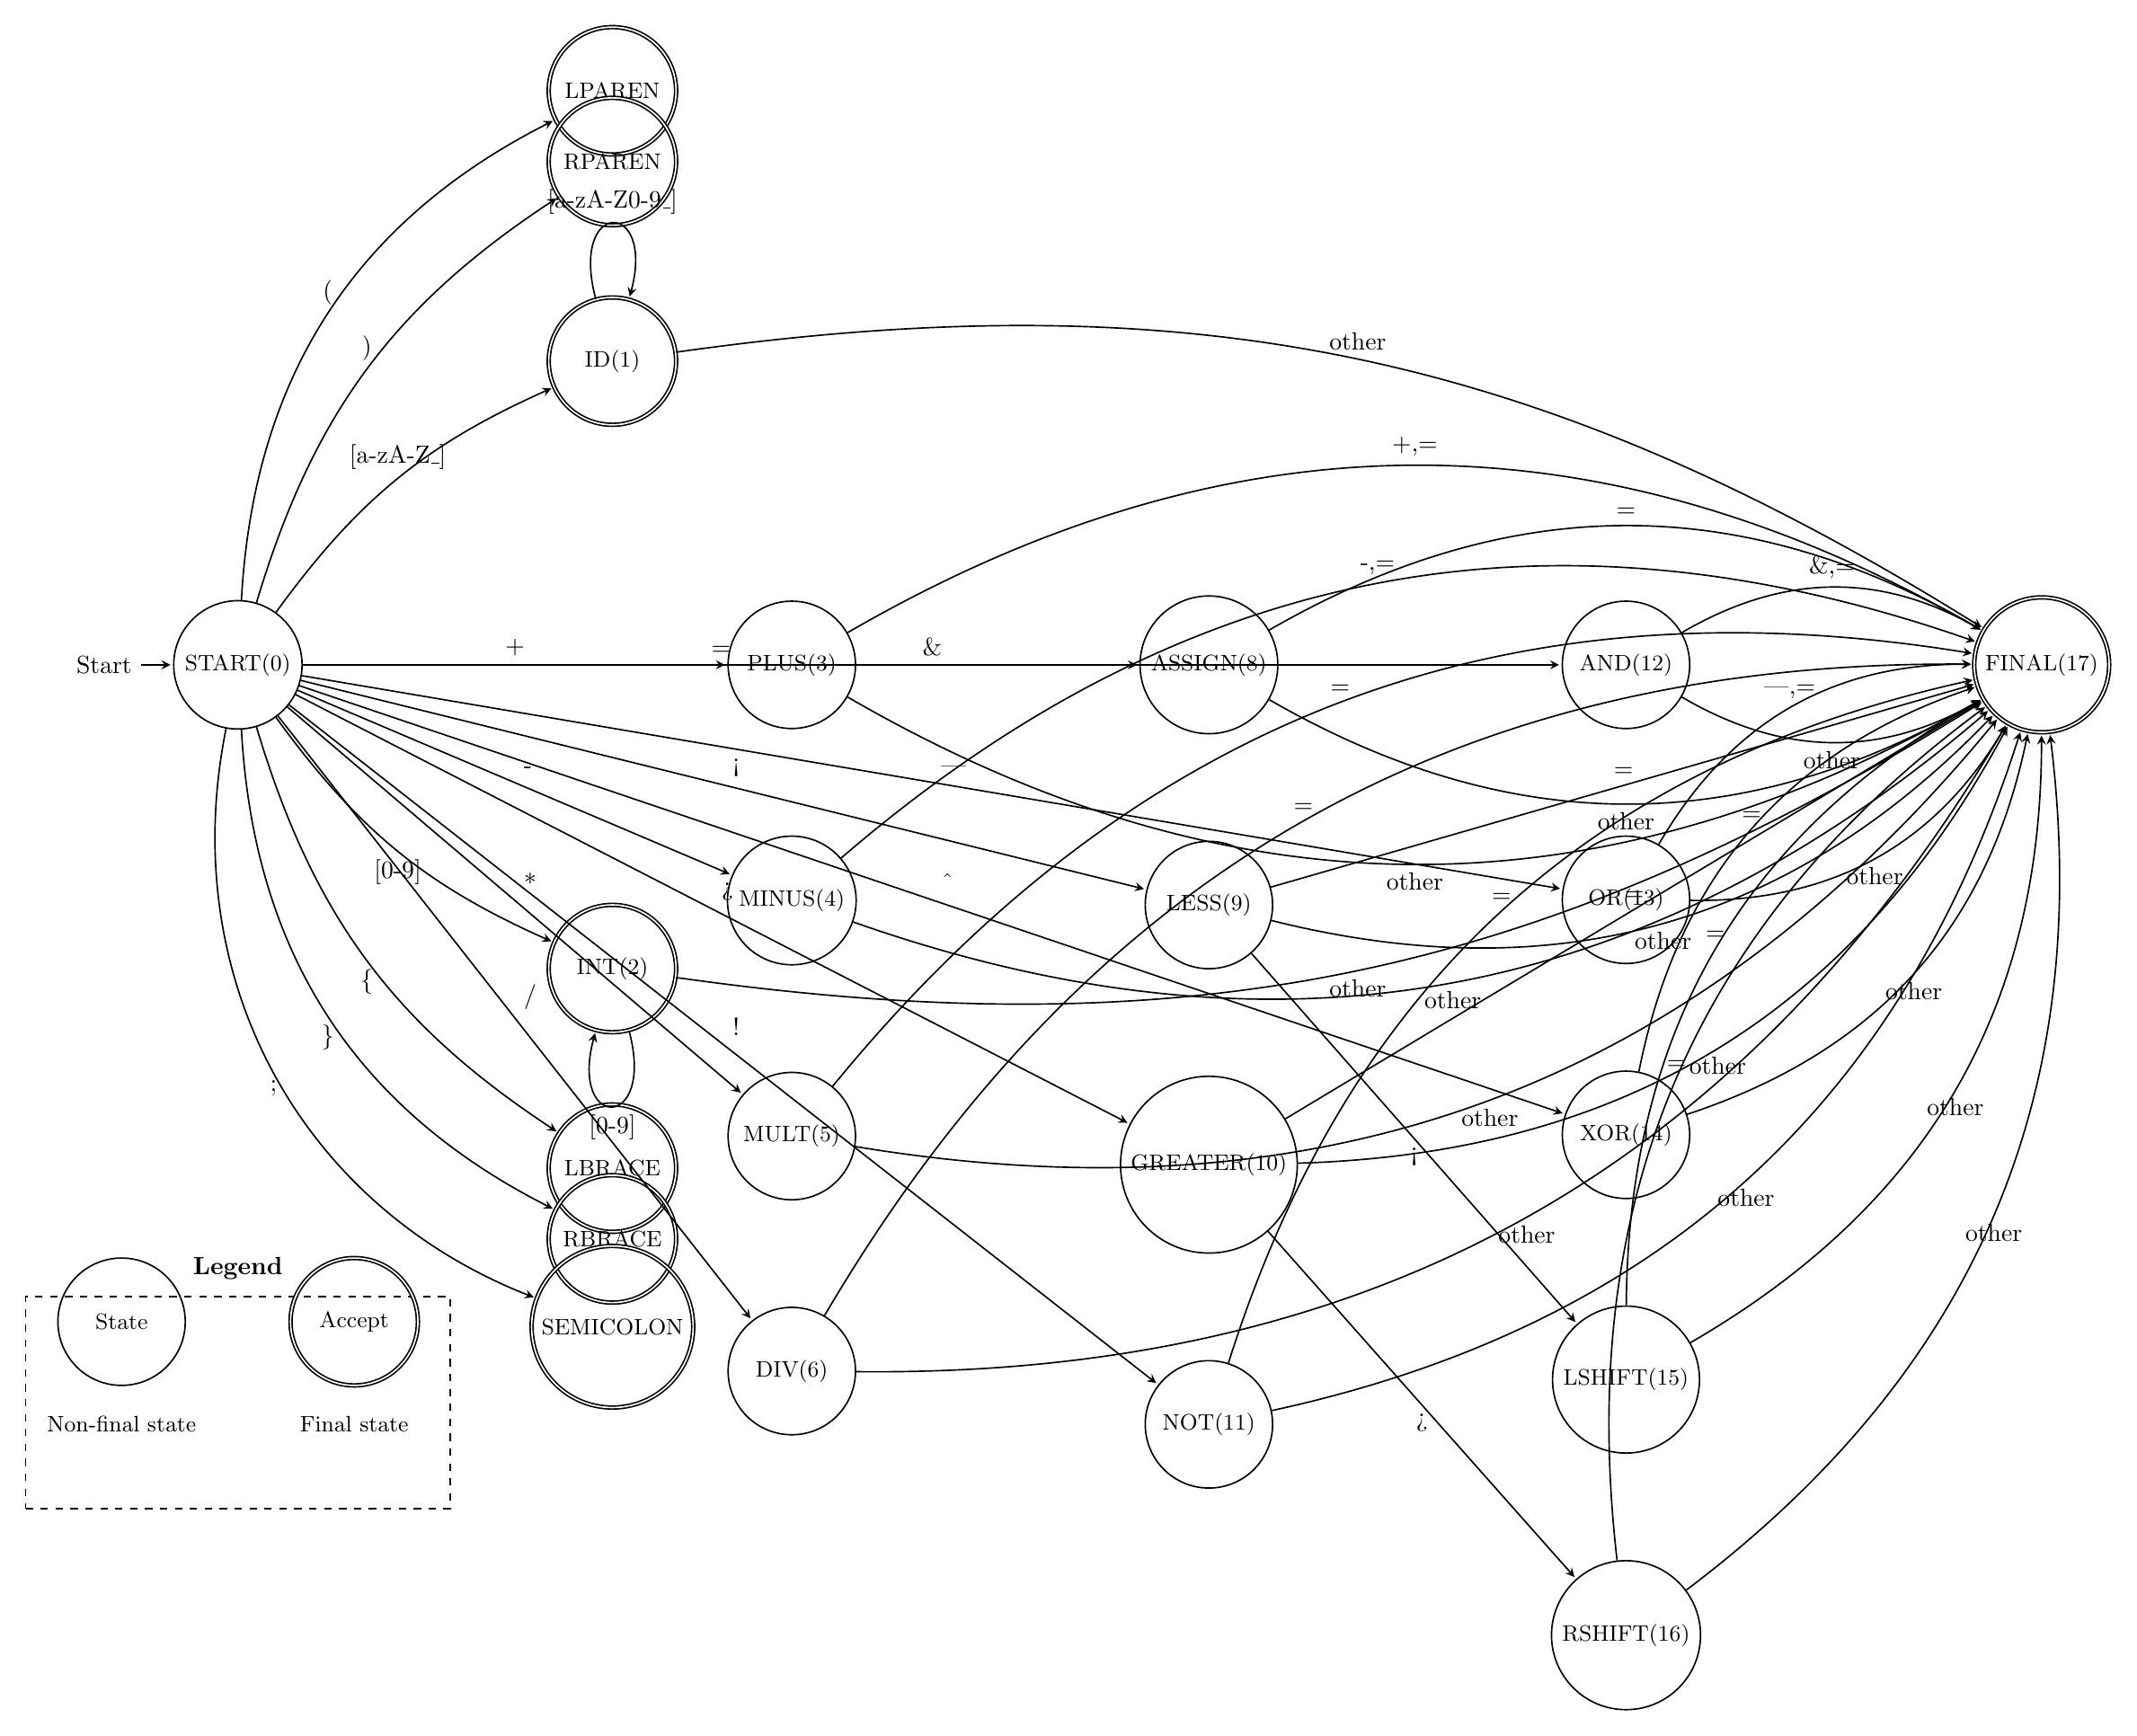
\begin{tikzpicture}[
    > = stealth,
    shorten > = 1pt,
    auto,
    node distance = 4cm,
    semithick,
    initial text=Start,
    state/.style={circle, draw, minimum size=1.8cm, font=\small},
    accept/.style={circle, draw, double, minimum size=1.8cm, font=\small},
    operator/.style={rectangle, draw, minimum width=2cm, minimum height=1cm, font=\small}
]

% Main states
\node[state, initial] (start) {START\\(0)};
\node[accept] (id) [above right=3cm and 4cm of start] {ID\\(1)};
\node[accept] (int) [below right=3cm and 4cm of start] {INT\\(2)};

% Operator states - arranged in a grid
\node[state] (plus) [right=6cm of start] {PLUS\\(3)};
\node[state] (minus) [below=1.5cm of plus] {MINUS\\(4)};
\node[state] (mult) [below=1.5cm of minus] {MULT\\(5)};
\node[state] (div) [below=1.5cm of mult] {DIV\\(6)};

\node[state] (assign) [right=4cm of plus] {ASSIGN\\(8)};
\node[state] (less) [below=1.5cm of assign] {LESS\\(9)};
\node[state] (greater) [below=1.5cm of less] {GREATER\\(10)};
\node[state] (not) [below=1.5cm of greater] {NOT\\(11)};

\node[state] (and) [right=4cm of assign] {AND\\(12)};
\node[state] (or) [below=1.5cm of and] {OR\\(13)};
\node[state] (xor) [below=1.5cm of or] {XOR\\(14)};
\node[state] (lshift) [below=1.5cm of xor] {LSHIFT\\(15)};
\node[state] (rshift) [below=1.5cm of lshift] {RSHIFT\\(16)};

% Final states
\node[accept] (final) [right=4cm of and] {FINAL\\(17)};

% Single character tokens (shown as final states)
\node[accept] (lparen) [above=2cm of id] {LPAREN};
\node[accept] (rparen) [above=1cm of id] {RPAREN};
\node[accept] (lbrace) [below=1cm of int] {LBRACE};
\node[accept] (rbrace) [below=2cm of int] {RBRACE};
\node[accept] (semicolon) [below=3cm of int] {SEMICOLON};

% Transitions from START
\path[->] 
    (start) edge [bend left=15] node [above] {[a-zA-Z\_]} (id)
    (start) edge [bend right=15] node [below] {[0-9]} (int)
    (start) edge node [above] {+} (plus)
    (start) edge node {-} (minus)
    (start) edge node {*} (mult)
    (start) edge node {/} (div)
    (start) edge node {=} (assign)
    (start) edge node {<} (less)
    (start) edge node {>} (greater)
    (start) edge node {!} (not)
    (start) edge node {\&} (and)
    (start) edge node {|} (or)
    (start) edge node {\^{}} (xor)
    (start) edge [bend left=30] node [above] {(} (lparen)
    (start) edge [bend left=20] node [above] {)} (rparen)
    (start) edge [bend right=20] node [below] {\{} (lbrace)
    (start) edge [bend right=30] node [below] {\}} (rbrace)
    (start) edge [bend right=40] node [below] {;} (semicolon);

% Self loops for ID and INT
\path[->]
    (id) edge [loop above] node {[a-zA-Z0-9\_]} (id)
    (int) edge [loop below] node {[0-9]} (int);

% Transitions to FINAL from ID and INT
\path[->]
    (id) edge [bend left=20] node [above] {other} (final)
    (int) edge [bend right=20] node [below] {other} (final);

% Operator transitions
\path[->]
    (plus) edge [bend left] node [above] {+,=} (final)
    (plus) edge [bend right] node [below] {other} (final)
    (minus) edge [bend left] node [above] {-,=} (final)
    (minus) edge [bend right] node [below] {other} (final)
    (mult) edge [bend left] node [above] {=} (final)
    (mult) edge [bend right] node [below] {other} (final)
    (div) edge [bend left] node [above] {=} (final)
    (div) edge [bend right] node [below] {other} (final)
    (assign) edge [bend left] node [above] {=} (final)
    (assign) edge [bend right] node [below] {other} (final);

% Complex operator transitions
\path[->]
    (less) edge node [above] {=} (final)
    (less) edge node [below] {<} (lshift)
    (less) edge [bend right] node [below] {other} (final)
    (greater) edge node [above] {=} (final)
    (greater) edge node [below] {>} (rshift)
    (greater) edge [bend right] node [below] {other} (final)
    (not) edge [bend left] node [above] {=} (final)
    (not) edge [bend right] node [below] {other} (final)
    (and) edge [bend left] node [above] {\&,=} (final)
    (and) edge [bend right] node [below] {other} (final)
    (or) edge [bend left] node [above] {|,=} (final)
    (or) edge [bend right] node [below] {other} (final)
    (xor) edge [bend left] node [above] {=} (final)
    (xor) edge [bend right] node [below] {other} (final)
    (lshift) edge [bend left] node [above] {=} (final)
    (lshift) edge [bend right] node [below] {other} (final)
    (rshift) edge [bend left] node [above] {=} (final)
    (rshift) edge [bend right] node [below] {other} (final);

% Legend
\node[rectangle, draw, dashed, minimum width=6cm, minimum height=3cm] (legend) [below=8cm of start] {};
\node[above=0.1cm of legend.north] {\textbf{Legend}};
\node[state] (leg_state) [above left=0.5cm and 1cm of legend.center] {State};
\node[accept] (leg_accept) [above right=0.5cm and 1cm of legend.center] {Accept};
\node[below=0.3cm of leg_state] {\small Non-final state};
\node[below=0.3cm of leg_accept] {\small Final state};

\end{tikzpicture}
\end{document}
